\documentclass[11pt,a4paper]{article}
\usepackage[spanish]{babel}
\usepackage[utf8]{inputenc}
\usepackage{amsmath}
\usepackage{amsfonts}
\usepackage{amssymb}
\usepackage{graphicx}
 \graphicspath{ {images/} }
\usepackage{makeidx}
\usepackage{verbatim} 
\begin{document}

\begin{titlepage}

\newcommand{\HRule}{\rule{\linewidth}{0.5mm}} 

\center

\textsc{\LARGE Universidad de Costa Rica}\\[1.5cm]
\textsc{\Large Escuela de Ciencias de la Computación e Informática}\\[0.5cm] 
\textsc{\large CI-1210 Diseño de Circuitos Digitales}\\[0.5cm] 

\HRule \\[0.4cm]
{ \huge \bfseries Una aproximación a la computación cuántica y el D-Wave como desarrollo de nuevos paradigmas computacionales}\\[0.4cm] % Title of your document
\HRule \\[1.5cm]

\begin{minipage}{0.4\textwidth}
\begin{flushleft} \large
\emph{Autores:}\\
Amanda \textsc{Sagasti}
Emmanuel \textsc{Arias} 
\end{flushleft}
\end{minipage}
~
\begin{minipage}{0.4\textwidth}
\begin{flushright} \large
\emph{Profesor:} \\
Sanders \textsc{Pacheco A.} % Supervisor's Name
\end{flushright}
\end{minipage}\\[4cm]

{\large 30 de Junio, 2014}\\[3cm] 

\vfill 

\end{titlepage}

%\tableofcontents 
%\clearpage


\part*{Introducción}

‘‘Computación cuántica’’ es un término popular en las noticias de avances tecnológicos hoy en día. Es una área de investigación que finalmente se puede realizar físicamente, después de años de desarrollarse teóricamente. Algunos creen que puede ser un gran avance y solucionar problemas complejos de gran magnitud, mientras otros creen que no hay diferencia alguna entre la computación clásica y la cuántica. 

Decidimos plantear nuestra investigación en tres áreas que se correlacionan. Exponemos cada una de ellas en tres partes distintas. La primera parte introduce los fundamentos, la segunda construye sobre las ideas del primer capítulo y la tercera expone un caso real de las computadoras cuánticas. 

En la parte I repasamos conceptos matemáticos para comprender las bases de la mecánica cuántica. No esperamos que el lector tenga conocimientos generales en álgebra lineal, aunque sería lo ideal. Por lo tanto este apartado introduce a grandes rasgos las bases algebraicas de las espacios vectoriales. Además, hacemos una pequeña introducción a la mecánica cuántica pero más que eso damos una visión específica de esta frente a la computación. Brevemente damos una perspectiva general histórica en los fundamentos más importantes de la computación contemporánea y planteamos cómo la mecánica cuántica puede ofrecer una respuestas a los problemas que se le han planteado a la computación clásica. 

En la parte II establecemos algunas diferencias entre la computación clásica y la computación cuántica, empezando por su unidad más básica: qubits. Luego ampliamos las diferencias a compuertas clásicas y su equivalente cuántico. Establecemos la importancia de dos efectos cuánticos: la superposición y el entrelazamiento y cómo estos afectan los qubits. Por último mencionamos la teletransportación cuántica y cómo puede ser una base para nuevos tipos de transferencia de datos.

En la última parte, pero no por eso menos importante exponemos una aplicación tangente de la computación cuántica. La compañía D-Wave Systems clama haber construido la primera computadora cuántica comercial de mundo. Nos parece interesante investigar sobre el nacimiento de esta y el desarrollo que han hecho en la computación cuántica. Luego nos enfocamos en la arquitectura de hardware que poseen sus computadoras, sus componentes básicos y el funcionamiento de estas. Finalmente, exponemos las posibles aplicaciones que podría tener la computación cuántica desde la visión de D-Wave Systems y además mencionamos algunos de los usuarios de las máquinas D-Wave.

\part{Conceptos Fundamentales}
\index{Conceptos Fundamentales}

En este capítulo vamos a desarrollar las bases necesarias para poder llegar a un pleno entendimiento de la investigación. Es una especie de marco teórico donde se abarcará la terminología básica de ciertos conceptos matemáticos y computacionales tratados en los siguientes capítulos. No debe entenderse como un glosario o un capítulo de definiciones sino que, este es el comienzo de la investigación en su etapa más básica.

\section*{Conceptos matemáticos}
 Para poder comprender mejor los postulados de la Teoría Cuántica es necesario tener un conocimiento básico de álgebra lineal, específicamente sobre espacios vectoriales. Asumimos que el lector posee conocimientos sobre este tema, sin embargo vamos a hacer un pequeño repaso en conceptos fundamentales. 
Shankar (1994) define los espacios vectoriales como:

\begin{quote}
\textit{Un espacio vectorial lineal $\mathbb{V}$ es una colección de objetos} $\vert1\rangle,\vert2\rangle,...,\vert V\rangle,...,\vert W\rangle,...,$ \textit{llamados vectores, para los cuales existe}
\\\\
1. Una regla definida para realizar la suma de vectores, denotada $\vert V\rangle+\vert W\rangle$
\\2. Una regla definida para la multiplicación por escalares \textit{a,b,...,} denotada $a\vert V\rangle$ con las siguientes características:
\\
\begin{itemize}
\item El resultado de estas operaciones resulta en otro elemento del espacio, una característica llamada \textit{cerrado}: $\vert V\rangle+ \vert W\rangle\in\mathbb{V}$.
\item La multiplicación por escalares es \textit{distributiva en los vectores}: $a(\vert V\rangle+\vert W\rangle)=a\vert V\rangle+a\vert W\rangle$.
\item La multiplicación por escalares es \textit{distributiva en los escalares}: $(a+b)\vert V\rangle=a\vert V\rangle+b\vert V\rangle$.
\item La multiplicación por escalares es \textit{asociativa}: $a(b\vert V\rangle)=ab\vert V\rangle$.
\item La suma es \textit{conmutativa}: $\vert V\rangle+\vert W\rangle=\vert W\rangle+\vert V\rangle$.
\item La suma es \textit{asociativa}: $\vert V\rangle+(\vert W\rangle+\vert Z\rangle)=(\vert V\rangle+\vert W\rangle)+\vert Z\rangle$.
\item Existe un \textit{vector nulo} $\vert 0\rangle$ que obedece $\vert V\rangle+\vert 0\rangle=\vert V\rangle$.
\item Para cada vector $\vert V\rangle$ existe un \textit{inverso respecto a la suma}, $\vert -V\rangle$, tal que $\vert V\rangle+\vert -V\rangle=\vert 0\rangle$. (p. 2)
\end{itemize}
\end{quote}

Esta notación de vectores $\vert V\rangle$ llamada \textit{notación Dirac} será muy utilizada más adelante cuando veamos los qubits, los cuales se rigen por las mismas reglas de espacios vectoriales mencionadas anteriormente. Además de estas reglas es necesario que consideremos los conceptos de \textit{campo}, \textit{combinaciones lineales} y \textit{bases ortonormales}.

Es importante que definamos el \textit{campo} de un espacio vectorial. El campo se refiere al espacio donde están definidos los escalares que multiplican al espacio vectorial. Como los vectores no son números en sí, estos no se pueden multiplicar. Entonces, para poder multiplicar vectores necesitamos usar escalar inscritos a un campo. Por ejemplo, un \textit{espacio vectorial real} es un espacio definido por escalares reales. De igual manera tenemos los \textit{espacios vectoriales complejos}, entre otros.

Debemos tener una noción básica de las combinaciones lineales en los espacios vectoriales. Como definición básica encontramos que Arce, Castillo y González (2003) explican que:
\begin{quote}
\textit{
Sea E un espacio vectorial y $\lbrace v_{1},v_{2},...,v_{p}\rbrace$, un conjunto de vectores de E. Se llama combinación lineal de los vectores $v_{1},v_{2},...,v_{p}$ al vector
\begin{center}
$v=a_{1}v_{1}+a_{2}v_{2}+\cdot\cdot\cdot+a_{p}v_{p}$
\end{center}
cualquiera sea la elección de los escalares $a_{1},a_{2},...,a_{p}$. Y al conjunto
\begin{center}
$\mathcal{C}\ell=\lbrace v_{1},...,v_{p}\rbrace = \lbrace a_{1}v_{1},a_{2}v_{2},...,a_{p}v_{p}\mid a_{1},a_{2},...,a_{p}\in\mathbb{R}\rbrace$
\end{center}
se le denomina conjunto de combinaciones lineales de $v_{1},v_{2},...,v_{p}$.(p. 221)
}
\end{quote}
Este concepto nos sirve además para comprender qué es una base. Se dice que:
\begin{quote}
\textit{Un conjunto de vectores $\lbrace v_{1},v_{2},..,v_{k}\rbrace$ de un espacio vectorial E, es una base de este espacio si y solo si todo vector $v \in E$ se puede expresar como combinación lineal \textbf{única} de los vectores $v_{1},v_{2},..,v_{k}$. (Arce et al., 2003, p. 226)
}
\end{quote}

Finalmente, para comprender el concepto de bases ortonormales necesitamos aclarar una operación de vectores y una característica de los mismos. Estas son el producto punto y la norma. El producto punto se define como:
\begin{quote}
\textit{
Sean $\vec{a}=(a_{1},a_{2},...,a_{n})^{t}$ y $\vec{b}=(b_{1},b_{2},...,b_{n})^{t}$. El producto escalar, o producto punto de $\vec{a}$ y $\vec{b}$ es un número real denotado y expresado en la siguiente forma:
\begin{center}
  $\vec{a}\cdot\vec{b}=a_{1}b_{1}+a_{2}b_{2}+\cdot\cdot\cdot+a_{n}b_{n}$ (Arce et al., 2003, p. 158)
\end{center}
}
\end{quote}
 Es decir, si tenemos dos vectores podemos multiplicar las entradas de estos en orden y la suma de estos dará un número real, o complejo dependiendo del campo. Debemos anotar que esta es la notación ordinaria de vectores. En la notación Dirac si tenemos los vectores \textit{V} y \textit{W} el producto punto está denotado como $\langle V\vert W\rangle$. Dos vectores son \textit{ortogonales o perpendiculares} si y solo si $\langle V\vert W\rangle=0$.
Por otro lado, la norma de un vector, también conocida como magnitud, de una forma generalizada se define por: "$\sqrt{\langle V\vert V\rangle}\equiv\vert V \vert$ (...). Un \textit{vector normal} tiene una norma igual a uno." (Shankar, 1994, p. 9)

Ahora bien, aclarados esto términos podemos definir una \textit{base ortonormal} como: $"$Un conjunto de vectores base normales, los cuales son ortogonales dos a dos." (Shankar, 1994, p. 9).

\section*{Introducción a la Mecánica Cuántica}

En cuanto al concepto de mecánica cuántica no discutiremos a profundidad los postulados que este propone, puesto que eso sería un enorme discusión. Sin embargo, vamos a comparar el primer postulado de la mecánica cuántica con el primer postulado de la mecánica clásica. El primero afirma que: ''El estado de una partícula en algún momento dado está especificado por las variables \textit{x(t)} y \textit{p(t)}, i.e., como un punto en un espacio de dos dimensiones.'' (Shankar, 1994, p. 115). Mientras que el segundo dice que: ''El estado de una partícula está representado por el vector $\vert \psi(t)\rangle$ en un espacio Hilbert.'' (Shankar, 1994, p.115)

Con este postulado, podríamos decir que tenemos la base para comprender el concepto de los qubits. Pero en general, ¿qué es la mecánica cuántica? Nielsen y Chuang (2010) la definen como: ''(...)un marco matemático o un conjunto de reglas para la construcción de teorías de la física.'' (p. 2). Nos parece contextualmente comprensible la analogía que plantean estos autores. En esta, comparan la relación que tiene la mecánica cuántica y las teorías que derivan de ella con un sistema operativo y sus aplicaciones de software (p. 2). Como vemos entre ambas relaciones hay una conexión de base, donde el primer concepto sirve de fundamento para que se creen los elementos con los cuales se relacionan.

Incluso yendo más allá de una simple definición y contexto histórico Nielsen y Chuang (2010) se atreven, luego de hacer una línea de tiempo en el desarrollo de la mecánica cuántica, a proponerla como un reto para la computación. Ellos exponen los inicios de esta nueva forma de ver la física, que se remontan a las años 20 hasta los hallazgos más destacables que datan desde los años 70 hasta la actualidad. Luego, hace una reflexión acerca de que los intentos por desarrollar nuevos hallazgos científicados, aunque sea por mera corazonada, han dado nacimiento a importantes descubrimientos en la historia de la humanidad. Es aquí donde ellos recalcan que la computación e informática cuántica caben a la perfección en este esquema de resolver retos propuestos por nuevos esquemas de conocimiento. (pp. 2-3)

Entonces, el desarrollo de la mecánica cuántica en las ciencias de la computación puede representar un inmenso avance en el desarrollo de soluciones para los problemas propios de este ciencia. 

Para poner un ejemplo, vamos a retroceder un momento en la historia y remontemos sobre los inicios de la computación. Si nos colocamos en los antecedentes de las primeras computadoras electrónicas tenemos el gran aporte de Alan Turing. Turing (1936) propone el concepto de una máquina que es capaz de interpretar un número finito de instrucciones llamadas "m-configurations". Esta máquina será alimentada por una cinta seccionada que va a contener el conjunto de instrucciones que se desean que la máquina interprete y como resultado imprimirá en otra cinta los resultados de las instrucciones que la máquina va a interpretar. (p. 232). Solo para recalcar la importancia del trabajo de Turing, Herken (1998) afirma que: ''Es bastante sorprendente ver cómo, en tan sólo diez años después de ''Computable Numbers'', había traducido sus ideas en una poderosa visión profética del potencial de la tecnología informática'' (p. 8) 

Volviendo a la línea histórica, tenemos el trabajo de Turing que mencionamos que data de 1936, seguido por el trabajo de John Von Neumann. Los aportes que Von Neumann hizo al conocimiento científico en general son muchos y en diversas áreas (incluyendo en la mecánica cuántica) pero ahora nos limitaremos a su trabajo \textit{First Draft of a Report on the EDVAC}. Incluso siendo una borrador incompleto, muestra la arquitectura de la computadora EDVAC. Esta se convirtió en la arquitectura más usada en la creación de nuevas computadoras y como base se ha mantenido hasta la actualidad. Con la invención del transistor en 1947 el desarrollo de nuevo hardware se vió impulsado y esta arquitectura obtuvo mucha más fuerza.

Gracias a los transistores, se comenzó el desarrollo de circuitos integrados. El experto en fisicoquímica Gordon Moore (1965) habla sobre las ventajas y los posibles usos de los circuitos integrados. Inclusive afirma que: 
\begin{quote}
el futuro de la electrónica integrada es el futuro de la electrónica misma.(...)

La electrónica integrada hará las técnicas electrónicas más accesibles al resto de la sociedad, realizando muchas funciones que en el presente se hacen inadecuadamente o no se hacen del todo. La principal ventaja serán bajos costos y diseños grandemente simplificados---recompensa de un suministro de paquetes funcionales de bajo costo. (pp. 1-2)
\end{quote}
 Sin embargo, él propone en este artículo una cierta preocupación. Moore (1965) esperaba que para la siguiente década se duplicara el número de componentes en un circuito integrado. Esta aproximación resulto ser casi apegada a la realidad del futuro tanto que se le dió el nombre de \textit{Ley de Moore}.

Con esto ya expuesto podemos tener una aproximación del futuro en la construcción de computadores a nivel de hardware. El crecimiento acelerado de componentes va a llegar a un punto donde va a ser necesario buscar una solución. Es aquí donde Nielsen y Chuang (2010) proponen como solución buscar nuevos paradigmas computacionales, y uno de estos puede ser fruto de la teoría de la computación cuántica. Los autores hablan sobre computadoras que procesen información usando métodos de mecánica cuántica a velocidad increíblemente rápidas en comparación con los métodos actuales con mecánica clásica. (pp. 4-5) Por tanto, decidimos investigar acerca de estos métodos de computación mediante mecánica cuántica. Como primera instancia, expondremos las unidades básicas y características fundamentales de la computación cuántica.
\clearpage
\part{Computación Cuántica}
\section*{Qubits}

Los quantum bits, o qubits, son objetos matemáticos que tiene dos posibles estados,  $\vert 0\rangle$ y $\vert 1\rangle$. La diferencia entre un qubit y un bit normal es que un qubit puede tener estados adicionales formados por combinaciones lineales de sus estados originales. (Nielsen, 2010, p.13)

Asumiendo que tenemos un espacio vectorial $\mathbb{C}$, podemos afirmar que los vectores $\vert 0\rangle$ y $\vert 1\rangle$ pertenecen a este espacio. En general, si queremos representar un qubit usamos la siguiente fórmula donde $\vert \psi \rangle$ es un vector que pertenece a $\mathbb{C}$:

\begin{center}
$\vert \psi \rangle = \alpha \vert 0\rangle + \beta \vert 1\rangle$
\end{center}

Los números $\alpha$ y $\beta$ son números complejos, aunque estos se pueden asumir como números reales. De otra manera, el estado de un qubit es un espacio vectorial complejo de dos dimensiones. Los estados $\vert 0\rangle$ y $\vert 1\rangle$ se conocen como ''estados base computacionales'' y forman una base ortonormal para este espacio vectorial. (Nielsen, 2010, p.13)

Podemos examinar un bit clásico para ver el valor que éste tiene. Por ejemplo, las computadoras revisan valores de bits constantemente al extraer contenidos de memoria. Sin embargo, no podemos examinar un qubit para determinar el estado en el que está. La mecánica cuántica nos dice que tenemos acceso solamente a información restringida sobre el estado cuántico de un qubit. Cuando medimos un qubit podemos tener dos posibles resultados: 0 con probabilidad $\alpha^2$ o 1 con probabilidad de $\beta^2$. La suma de ambas probabilidades debe dar 1. Geométricamente, podemos interpretar esto como la condición en la cual el estado del qubit se normaliza a 1. En general, el estado de un qubit es un vector unitario en un espacio vectorial complejo de dos dimensiones.  (Nielsen, 2010, p.13)

La habilidad de un qubit de estar en un estado superpuesto va en contra del entendimiento clásico del mundo que nos rodea. Un qubit puede existir en un continuo de estados entre $\vert 0\rangle$ y $\vert 1\rangle$ hasta que es observado. Cuando se observa un qubit, su medición es '0' o '1'. (Nielsen, 2010, p.14)

Los qubits son reales, y varios sistemas físicos se pueden utilizar para hacer qubits. Por ejemplo, se pueden realizar con las dos distintas polarizaciones de un fotón, con el alineamiento del espín nuclear en un campo magnético uniforme, como dos estados de un electrón orbitando un átomo. (Nielsen, 2010, p.14) 

La representación geométrica de un qubit se puede apreciar en la Figura 1.

\begin{figure}
\centering
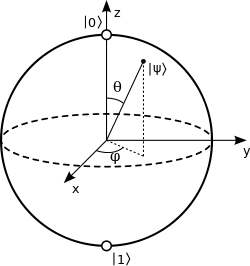
\includegraphics[width=0.45\textwidth]{qubit}
\caption{Representación geométrica de un qubit (wikimedia.org)}
\end{figure}

Los cambios que le suceden a un estado cuántico se pueden describir usando la computación cuántica. De la misma manera que una computadora clásica está construida con base en circuitos lógicos, una computadora cuántica se basa en circuitos cuánticos con compuertas cuánticas elementales.
 
\section*{Compuertas con un qubit}

Consideremos la operación lógica NOT que modifica un bit clásico. Es una operación que no pierde información y es reversible con otro NOT. (Feynman, 1985, p.12)
Su tabla de verdad está descrita en el Cuadro 1.

Cuadro 1: Tabla de verdad de NOT
\begin{center}
    \begin{tabular}{ c | c }
    x & NOT x \\ 
	\hline
    0 & 1\\ 
    1 & 0 \\ 
    \end{tabular}
\end{center}

Al usar qubits, tener un NOT que cambie de $\vert 0\rangle$ a $\vert 1\rangle$ y viceversa no establece qué sucede en los estados de superposición. 
El NOT funciona de una manera lineal porque toma el estado 
 $\alpha \vert 0\rangle + \beta \vert 1\rangle$
 y lo modifica hasta que los papeles del $\vert 0\rangle$ y $\vert 1\rangle$ estén completamente intercambiados. 
  $\alpha \vert 1\rangle + \beta \vert 0\rangle$. 
Las compuertas cuánticas NOT se pueden describir en matrices de 2x2 (surge directamente de la linealidad). Supongamos que la X representa una compuerta NOT. 
$X \equiv \begin{bmatrix}
		\ 0 & 1 \\
		\ 1 & 0 \\
	      \end{bmatrix}$
Si escribimos el estado cuántico $\alpha \vert 0\rangle + \beta \vert 1\rangle$ en notación vectorial
$
\begin{bmatrix}
 \ \alpha \\
 \ \beta
 \end{bmatrix}
$
la salida del NOT cuántico es 
$X \begin{bmatrix} 
     \ \alpha \\
     \ \beta  \\
 \end{bmatrix}
 = \begin{bmatrix}
 \ \beta  \\
 \ \alpha \\
 \end{bmatrix}$.
 
La acción de un NOT es tomar el estado 0 y reemplazarlo por el estado correspondiente a la primera columna de la matriz X. De igual manera el estado 1 es reemplazado por el estado correspondiente a la segunda columna de la matriz X. 

Hay dos otras compuertas de un qubit importantes. 
La primera es la compuerta Z. 
$Z = \begin{bmatrix}
 \ 1 & 0  \\
 \ 0 & -1 \\
 \end{bmatrix}$.
Esta compuerta deja el 0 sin modificar y cambia el signo de 1 a -1.

La segunda es la compuerta Hadamard.
$H =  \frac{1}{\sqrt{2}}  \begin{bmatrix}
             \ 1 & 1 \\
             \ 1 & 1 \\
           \end{bmatrix}$.

\section*{Compuertas con múltiples qubits}
\subsection*{CONTROLLED NOT}

En un CONTROLLED NOT entran dos datos, \textit{a} y \textit{b}, y salen dos datos \textit{a'} y \textit{b'}. \textit{a} es la línea de control: si se activa y \textit{a}=1, entonces \textit{b'} es la negación de \textit{b}. Si \textit{a}=0, entonces \textit{b}=\textit{b'}. La acción de un CONTROLLED NOT es revertida al aplicar un CNOT de nuevo. 
La salida \textit{b'} es en realidad una función simétrica de \textit{a} y \textit{b} conocida como XOR. Es a la vez la suma módulo dos de \textit{a} y \textit{b}. Se puede utilizar para comparar los valores de \textit{a} y \textit{b} y dar como resultado 1 cuando son diferentes. (Feynman, 1985, p.12)

\subsection*{CONTROLLED CONTROLLED NOT}

En este caso hay dos líneas de control a y b que modifican a la tercera línea c y le aplican un NOT sólo cuando ambas líneas de control están activadas (a=1 y b=1). Si no, la salida c' se mantiene inmutada. (Feynman, 1985, p.12)

El CNOT y las compuertas de un qubit son los prototipos necesarios para hacer cualquier otro tipo de compuerta (son el NAND de los bits clásicos). (Nielsen, 2010, p.22)

\section*{Circuitos cuánticos}

¿Podemos simular circuitos con compuertas clásicas usando circuitos cuánticos? La respuesta es sí. Sin embargo, la mayoría de las compuertas cuánticas son reversibles, mientras las compuertas clásicas son irreversibles. (Nielsen, 2010, p.29)
Cualquier circuito clásico puede ser reemplazado por uno equivalente construido únicamente con elementos reversibles, utilizando la \textit{compuerta Toffoli}. La compuerta Toffoli tiene tres bits de entrada y tres de salida. Dos de esos bits son de control y no los afecta la acción de la compuerta en sí. El tercero es un bit que es "flippeado" , si las dos líneas de control están activadas. Aplicar dos veces la compuerta Toffoli a un bit hace que se revierta al estado original porque su inversa es sí misma. (Nielsen, 2010, p.29)
La compuerta Toffoli se puede utilizar para simular compuertas NAND. (Nielsen, 2010, p.29)

\section*{Superposición y Entrelazamiento cuántico}

El entrelazamiento cuántico es uno de los fenómenos más extraños y sorprendentes de la mecánica cuántica. No es un concepto nuevo, la propuesta del entrelazamiento se remonta hacia los años 30 donde la teoría cuántica comenzaba a desarrollarse. 

Para hacerlo de una forma comprendible vamos a referirnos a la analogía propuesta por Aczel (2001). Esta nos propone que imaginemos que Alice y Bob están casados. Cuando Alice se va de viaje Bob conoce a Carol. Carol está casada con Dave, quién también está fuera de la ciudad. Entonces Bob y Carol se olvidan de sus esposos y se entrelazan profundamente. Por una extraña razón Alice y Dave se encuentran y ellos también se entrelazan sin siquiera saber por qué. Entonces si cambiamos las personas por partículas: A, B, C, D y si sabemos que A está entrelazada con B al igual que C con D  entonces podemos entrelazar A con D por medio de entrelazar a B con C. (p. 2)

Por tanto, si dos partículas están entrelazas, no importa cuán lejos estén siempre van a estar unidas. Hay una relación intrínseca entre las dos que no las deja separarse. El entrelazamiento viene a ser entonces una aplicación de un concepto desarrollado en el pasado llamado el \textit{principio de superposición de estados}. Aczel (2001) lo presenta como:
\begin{quote}
El principio de superposición dice que un nuevo estado de un sistema puede estar compuesto por dos o más estados, de manera tal que el nuevo estado comparta algunas de las propiedades de los estados combinados. Si A y B atribuyen dos propiedades diferentes a una partícula, como la de estar en dos distintos lados, entonces la \textit{superposición} de estados, escrita como $A + B$, tiene algo en común con el estado A y el estado B. En particular, la partícula tendrá probabilidades distintas de cero de estar en cada uno de los dos estados, pero no en otra parte, si la posición de la partícula es observada. (p. 25)
\end{quote}
El entrelazamiento consiste en un sistema formado por dos o más subsistemas. En este caso el subsistema corresponde a una partícula. Veamos entonces qué significa decir que dos partículas están entrelazadas. Supongamos una partícula 1. Esta puede estar en dos estados: A y C. Estos estados manifiestan dos propiedades contradictorias como lo es el estar en dos lugares a la vez. Por otro lado, la partícula 2 puede estar en dos estados: B y D. De igual forma estos dos estados presentar la propiedad contradictoria de estar en dos lugares distintos. El estado AB es un producto de estados. Cuando el sistema completo esta en AB sabemos que la partícula 1 esta en A y la partícula 2 está en B. Analógicamente, con el estado CD. Observemos entonces el estado $AB + CD$. Este estado representa la aplicación del principio de superposición en todo el sistema de dos partículas. Como el principio permite este comportamiento de combinación de estados, el estado $AB + CD$ es llamado un \textit{estado entrelazado}. (Aczel, 2001, p. 26)

\section*{Teletrasportación cuántica}

A veces, la ciencia ficción deja de ser ficción para convertirse en tecnología del presente. Muchos recordarán la serie \textit{Star Trek} y como el Capitán Kirk era teletransportado a la nave \textit{Enterprise} com su famosa frase: \textit{''Beam me up Scotty''}. Este tipo de ideas, que un principio existen solo en la ficción pasan a ser investigadas en tangenciales campos científicos. En el apartado anterior desarrollamos el concepto de entrelazamiento cuántico por un motivo. Gracias a esta propiedad de las partículas cuánticas se ha logrado la \textit{teletransportación cuántica}. 

Los inicios de la teletransportación se remontan a los años 80 cuando William Wootters y W. Zurek presentan el \textit{Teorema del no clonado}, el cual muestra que una partícula cuántica no puede ser clonada. El teorema dice que, si tenemos una partícula, es imposible copiar su estado en otra, mientras la partícula original permanezca igual.  Por tanto, no se puede tener una especie de dispositivo que copie las propiedades de una partícula en otra. La solución dada a este problema por los físicos fue la de imprimir el estado de una partícula en otro y hacerla desaparecer en la original. Este proceso es el que se conoce como \textit{teletransportación}  (Aczel, 2001, p. 242)

En 1997, un grupo de físicos lograron con éxito un experimento donde pudieron teletransportar cuánticamente una partícula. Su experimento fue publicado en un artículo de la prestigiosa revista \textit{Nature}. Este dice:
\begin{quote}
El sueño de la teletransportación es el de ser capaz de viajar simplemente reapareciendo en un lugar distante. Un objeto que se ha teletransportado puede ser totalmente caracterizado por sus propiedades, que en la física clásica se pueden determinar mediante la medición. (Bouwmeester et al., 1997)
\end{quote}

El problema de la teletransportación de una partícula cuántico bajo este esquema clásico es que no puede ser medida con precisión. Esté es el principio de incertidumbre de Heisenberg. Si una partícula es medida u observada en el momento de teletransportarse, se destruirían todos sus otros estados y la precisión de la medición es improbable. Entonces, el artículo destaca que Bennett et al. propone la posibilidad de transferir un estado cuántico de una partícula en otra sin tener que obtener información en el proceso. Proponen que esto es posible gracias al entrelazamiento. (Bouwmeester et al., 1997)

Explicar el proceso por el cual se logra transferir el estado de una partícula a otro a es algo complicado. Decidimos entonces exponer una aplicación de directa de la computación cuántica en la computación e informática. Si pudieramos tranferir el estado de un qubit a otro podríamos tener un nuevo sistema de envío de datos. En el periódico \textit{The New York Times} encontramos una noticia sobre un grupo de científicos de los Países Bajos lograron teletransportar la información de un qubit a otro estando a tres metros de distancia. Este logro los motiva a continuar sus esfuerzo por lograr una teletransportación a distancias más largas. Si lo logran, este será un paso muy grande para la demostración del fenómeno del entrelazamiento y la mecánica cuántica en general. (Markoff, 2014)
\clearpage
\part{D-Wave Systems}
\section*{Historia y objetivos de D-Wave Systems}

D-Wave Systems es la primera compañía privada comercial que ofrece computación cuántica. Se basa en los principios de que la computación cuántica tiene el potencial de resolver algunos de los problemas más complejos alrededor del mundo. Esperan que la computación cuántica pueda llevar a nuevos descubrimientos en ciencia, ingeniería, modelos en computación, simulación, análisis financiero, optimización, lógica...

Fue fundada en 1999 por Geordie Rose, Haig Farris y Alexandre Zagoskin, que se encontraron en la Universidad de British Columbia (UBC). El nombre D-Wave viene de los primeros diseños de qubits que plantearon, que usaban superconductores de tipo d-wave. Empezó como una rama de UBC con lazos muy fuertes con el Departamento de Física y Astronomía, ya que ellos proporcionaban los fondos para investigación en la computación cuántica. El objetivo de D-Wave es integrar nuevos descubrimietos en física y computación para producir nuevos avances en la computación cuántica.

Por cinco años la companía trabajó para recopilar propiedad intelectual e ideas de cómo la computación cuántica podía volverse una realidad. Más que investigación académica, estaban enfocados en cómo diseñar las computadoras cuánticas, cuál es el proceso de manufactura y cómo se pueden producir en masa. 
Para el 2004, después de varios intentos de buscar opciones de terceros para construir las computadoras, tomaron la decisión de construir las computadoras ellos mismos. Construyeron sus propias facilidades para producir las partes necesarias y los procesadores que simulaban efectos cuánticos. También armaron un equipo de científicos para diseñar, fabricar y probar los procesadores en sus propios laboratorios. 

En el 2010 lanzaron la primera computadora cuántica comercial, la D-Wave One, y para el 2013 lanzaron la D-Wave Two, que tiene 512 qubits. Instalaron la D-Wave Two en los laboratorios de Inteligencia Artificial Cuántica administrados por Google, NASA y USRA. 

Hoy en día es reconocida como una de las compañías pioneras en computadoras cuánticas basadas en superconductores. Fue nombrada como una de las 50 compañías más inteligentes de acuerdo al MIT Technology Review de este año. Tiene más de 100 patentes y sus sistemas son utilizados por organizaciones reconocidas mundialmente. Tienen varias oficinas: Vancouver, Canada; Palo Alto, California y Washington DC. 

\section*{La computadora Cuántica D-Wave}
\subsection*{Introducción a la computadora D-Wave}

La computadora D-Wave utiliza los principios de la mecánica cuántica para resolver problemas computacionales. Gracias a los algoritmos cuánticos es posible resolver tareas complejas en un tiempo mucho menor que con una computadora clásica. La computadora D-Wave no hace todas las operaciones que hace una normal, sino que está construida especialmente para resolver problemas de optimización. (D-Wave Systems, 2014)

Entonces, ¿cúal es la diferencia entre una computadora cuántica y una computadora clásica? D-Wave Systems expone una analogía entre estas estructuras. Imaginemonos un mapa con valles y montañas. Resolver un problema de optimización sería como encontrar el punto más bajo en este mapa. Una computadora clásica utilizaría un algoritmo que recorrería todos los puntos posibles del mapa y los analiza hasta luego conseguir el mejor resultado. El procesamiento de la D-Wave es capaz de considerar todas las posibilidades al mismo tiempo y le devuelve al usuario un conjunto que incluye no solo al mejor resultado sino a otros resultados también. (D-Wave Systems, 2014)

Siguiendo este ejemplo, si un usuario quisiera resolver este problema, primero expresa su problema en un lenguaje adecuado a D-Wave y se conectaría a la computadora mediante una red, como si fuera un dispositivo periférico. Luego de enviar el problema, la máquina se encarga de hacer operaciónes cuánticas para luego darle al usuario la respuesta al problema.  (D-Wave Systems, 2014)

La computadora D-Wave es capaz de resolver problemas como por ejemplo: optimización, análisis financiero, aprendizaje de máquina, reconocimiento de patrones, detección de anomalías, verificación de software y hardware, entre otras. (D-Wave Systems, 2014) Vemos que las aplicaciones son muy enriquecedoras en ciertos campos, tanto como científicos, comerciales y militares, por lo que dedicaremos un apartado más adelante a estas posibles aplicaciones.

\subsection*{Hardware del D-Wave}

Para hablar un poco sobre la mecánica del hardware del D-Wave vamos a referirnos a tres entornos: adentro del procesador, afuera del procesor y la máquina en general.

En cuanto al procesador hay una singularidad importante. En una computadora clásica, la forma en la que se almacenan los bits es mediante transistores. Estos están conectados a un bus de datos y la forma en que se escriben los datos es regulando el voltaje en los transistores. En cambio, el D-Wave necesita un medio para almacenar qubits, y un transistor no se puede utilizar. Entonces, el procesador esta conformado por una unidad básica llamada SQUID. En esta estructura los electrones pueden comportarse en forma de onda, las cuales dan las propiedades y efectos cuánticos. En contraste con un transistor que está hecho de silicio, este dispositivo está hecho de niobio. Cuando este metal se enfría se transforma en un superconductor, permitiéndo que fluya en el propiedades cuánticas.(D-Wave Systems, 2014)

Para ser más gráficos, en la siguiente figura tenemos respectivamente un transistor CMOS y un SQUID (nombre que se le da al dispositivos que almacena quibts en el D-Wave):

\begin{figure}[h]
\centering
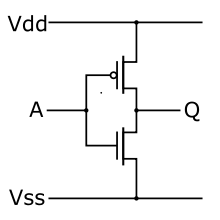
\includegraphics[width=0.45\textwidth]{cmos}
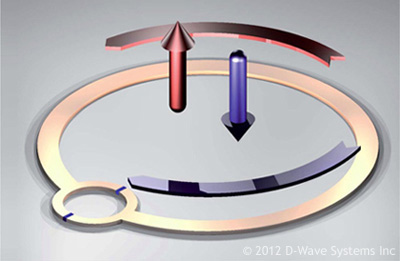
\includegraphics[width=0.45\textwidth]{squid}
\caption{Esquemas de un transistor CMOS y un SQUID (wikipedia.org, 2014) (D-Wave Systems, 2014)}
\end{figure}

En el CMOS podemos ver que tenemos las entradas para los voltajes que hacen que el transistor almacene cierto estado. En el SQUID el anillo de niobio y dos flechas, estas corresponden a un campo magnético. A las direcciones de este campo se les conoce como +1 y -1. En estos estados se puede plasmar la superposición de un qubit en sus dos estados.

Estos quibts se acomodan en un serie de acoples hechos de material superconductor para poder tener un circuito de qubits programables. Para mapear estos qubits se utilizan switches con los cuales se les asignan direcciones. (D-Wave Systems, 2014)

Una vez que se tuvo diseñado el circuito del procesador y de hacer los esquemas, se comienza la manufactura del mismo. Para esto, se usó una galleta de silicio para colocar todos los componentes. Como vemos el proceso se asemeja al de la manufactura de un procesador clásico. (D-Wave Systems, 2014) En la siguiente figura vemos un procesador de un D-Wave One.
\clearpage
\begin{figure}
\centering
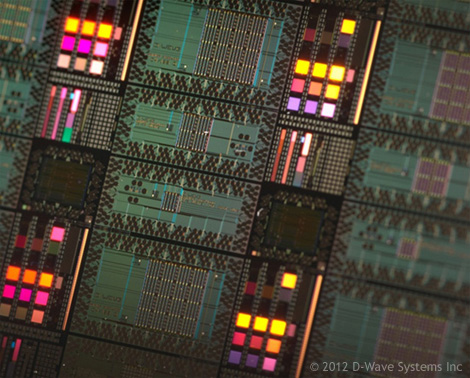
\includegraphics[width=0.45\textwidth]{proce}
\caption{Fotografía de una galleta de procesadores Rainier, incluyendo el procesador de 128 qubits usado en el D-Wave One (D-Wave Systems, 2014)}
\end{figure}

Para construir la computadora, se toma uno de estos procesadores y se empaqueta en un sistema de circuitos que mantiene todas las conexiones. Para que este procesador funcione se necesita que se enfríe a una temperatura sumamente baja. Se requieren aproximadamente 80 mK ($-273^o$C). Esta temperatura es 150 veces más fría que el espacio interestelar, solo $0.02^o$C por encima del cero absoluto. Esta temperatura se logra usando helio como enfriador. El líquido reside en una cámara por aparte y el procesador se enfría "en seco". La refrigeración es viable y mantenible comercialmente. (D-Wave Systems, 2014)

El procesador es afectado directamente por campos magnéticos, por lo que D-Wave tiene sumo cuidado con estos. La computadora crea un escudo de campos magnéticos que contrarestan en su totalidad los campos magnéticos que puedan quere atravesar el cajón donde está el procesador. (D-Wave Systems, 2014)

En referencia al contenedor de la computadora, además de tener el escudo magnético tiene además una protección contra radiofrecuencias electromagnéticas. Más aún, solo hay una salida del cajón con el exterior y es un canal óptico por el cual los datos entran y los resultados salen.  (D-Wave Systems, 2014)

Si vemos un D-Wave en su totalidad observamos una gran caja negra. Este contenedor tiene el espacio donde está el procesador además de los gabinetes donde van los sistemas de enfriamiento y el sistema de control. La siguiente figura muestra dos D-Wave One.
\clearpage
\begin{figure}
\centering
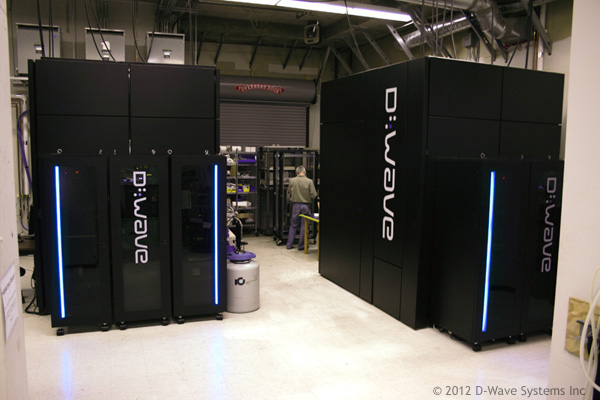
\includegraphics[width=0.45\textwidth]{dwave}
\caption{Dos D-Wave One siendo probados en el laboratorio (D-Wave Systems, 2014)}
\end{figure}

El método de conexión al D-Wave se basa en computación en nube. El D-Wave tiene su propio servido que tiene una cola de tareas por hacer. Este modelo permite que este tipo de computación sea muy accesible a un gran número de personas. En la figura anterior vemos el esquema que tiene un D-Wave en una conexión de área local.

\begin{figure}
\centering
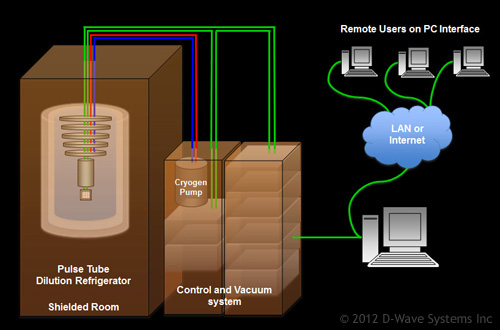
\includegraphics[width=0.45\textwidth]{esquema}
\caption{Esquema de conexión de un D-Wave (D-Wave Systems, 2014)}
\end{figure}

\clearpage
\subsection*{Aplicaciones y usuarios del D-Wave}

Como ya lo habíamos mencionado, el D-Wave se centra en problemas de optimización. Pero en general D-Wave Systems nos da varios ejemplos de este tipo de problemas. Por ejemplo, se podría optimizar redes de tuberías de agua. Con un software se modelan las especificaciones y la computadora se encargaría de ofrecer la mejor solución. Otro problema es el de optimizar las dosis de radioterapia en un paciente. Como esto lleva muchas variables a considerar para que el tratamiento tenga el menor impacto en el cuerpo, la capaciadad de procesamiento de la computación cuántica podría ser un gran avance.(D-Wave Systems, 2014)

En el campo de la ciencia tenemos el ejemplo de analizar el plegamiento de las proteínas. Con la computación cuántica se pueden explorar los posibles plegamientos que pueden tener estas moléculas. D-Wave en conjunto con investigadores de la universidad de Harvard diseñaron un sistema que predice los patrones de plegamiento de proteínas y han logrado pequeñas simulaciones. (D-Wave Systems, 2014)

Con respecto a la robótica se podría usar la computación cuántica para aprender compotamiento y procesar imágenes y video. Uno de los limitantes de los programadores actualmente es la dificultad de desarrollar algoritmos que hagan que una máquina aprenda comportamientos. Como el procesamiento de grandes árboles de datos es un problema para las computadoras clásicas, la capacidad de optimización de la computación cuántica puede ser útil en este caso. (D-Wave Systems, 2014)

Y cuáles industrias podrían estar interesadas en la computación cuántica. Podríamos mencionar universidades, laboratorios, compañias financieras, compañías energéticas, defensa y militares y hasta la misma web. (D-Wave Systems, 2014)

Actualmente, D-Wave tiene clientes importantes, uno de ellos es la NASA y Google. Estos, en colaboración con la Asociación de Universidades de Investigación Espacial crearon en el 2013 el Laboratorio Cuántico de Inteligencia Artificial (QuAIL siglas en inglés). Google se centra en mejorar modelos de optimización con la computación cuántica. La NASA intenta demostrar que tanto esta como los algoritmos cuánticos pueden cambiar tareas de optimización como reconocimiento de patrones, tráfico aéreo, navegación, robótica, comunicaciones entre otros. (D-Wave Systems, 2014)

El primer cliente de D-Wave fue Lockheed Martin. Es uno de los contratistas en defensa más grande del mundo. Con la D-Wave logró identificar en seis semanas un error en una pieza de código de un F-16 de hace 30 años que le tomo a su compañia meses en averiguar. Martin trabaja en Aeronaútica, Sistemas de Información y soluciones militares. Él disela systemas complejos, aunque mucho del trabajo pesado consiste en verificar y validar. El grupo de trabajo de Martin intenta reducir el costo y tiempo de este trabajo con la computación cuántica.

El D-Wave que compró Martin, cabe destacar que fue el primer D-Wave comercialmente disponible, está en el Instituto de Ciencias de la Información de la Universidad del Sur de California. Este instituto está posicionado a la cabeza de la investigación en computación cuántica.

\part*{Conclusión}


\clearpage
\begin{thebibliography}{X}
\index{Referencias}
\bibitem{etiqueta} \textsc{Autor, A.} (año). \textit{Título del libro.} Lugar: Editorial
\bibitem{revistaonline} \textsc{Autor, A.} (año). Título del artículo. \textit{Revista}, n, pp. doi: (o recuperado de)
\bibitem{periodico} \textsc{Autor, A.} (año). Título de la notica. \textit{Periodico} Recuperado de
\bibitem{aczel} \textsc{Aczel, A.} (año). \textit{ENTANGLEMENT The Greatest Mystery in Physics.} New York: Four Wall Eight Windows
\bibitem{arce} \textsc{Arce, C., Castillo, W., González, J.} (2003). \textit{Álgebra Lineal.} Lugar: Editorial
\bibitem{bouwmeester} \textsc{Bouwmeester, D., Pan J., Mattle K., Eibl M., Weinfurter H., Zeilinger A.} (1997). Experimental quantum teleportation. \textit{Nature}, 390, 575-579. doi:10.1038/37539
\bibitem{dwave2} \textsc{D-Wave Systems} (2014). Applications. Recuperado de http://www.dwavesys.com/quantum-computing/applications
\bibitem{dwave4} \textsc{D-Wave Systems} (2014). Customers. Recuperado de http://www.dwavesys.com/our-company/customers
\bibitem{dwave3} \textsc{D-Wave Systems} (2014). Industries. Recuperado de http://www.dwavesys.com/quantum-computing/industries
\bibitem{dwave6} \textsc{D-Wave Systems} (2014). Introduction to the D-Wave Quantum Hardware. Recuperado de http://www.dwavesys.com/tutorials/background-reading-series/introduction-d-wave-quantum-hardware
\bibitem{dwave1} \textsc{D-Wave Systems} (2014). Quantum Computing. Recuperado de http://www.dwavesys.com/quantum-computing
\bibitem{dwave5} \textsc{D-Wave Systems} (2014). The D-Wave Two System. Recuperado de http://www.dwavesys.com/d-wave-two-system
\bibitem{feynman} \textsc{Feynman, R.} (1985). \textit{Quantum Mechanical Computers.} Recuperado de $http://www.cs.princeton.edu/courses/archive/fall05/frs119/papers$
$/feynman85_optics_letters.pdf$
\bibitem{herken} \textsc{Herken, R. (Ed.)} (1988). \textit{The Universal Turing Machine. A Half-Century Survey.} Oxford University Press
\bibitem{markoff} \textsc{Markoff, J.} (2014). Scientists Report Finding Reliable Way to Teleport Data. \textit{The New York Times} Recuperado de http://www.nytimes.com/2014/05/30/science/scientists-report-finding-reliable-way-to-teleport-data.html
\bibitem{moore} \textsc{Moore, G.} (1965). Cramming more components onto integrated circuits. \textit{Electronics.} Vol 3., No. 8.
\bibitem{nielsen} \textsc{Nielsen, M., Chuang, I.} (2010). \textit{Quantum Computation and Quantum Information.} New York: Cambridge University Press
\bibitem{shankar} \textsc{Shankar, R.} (1994). \textit{Principles of Quantum Mechanics.} New York: Plenum Press
\bibitem{turing} \textsc{Turing, A.} (1936). \textit{ON COMPUTABLE NUMBERS, WITH AN APPLICATION TO
THE ENTSCHEIDUNGSPROBLEM.} Recuperado de http://classes.soe.ucsc.edu/cmps210/Winter11/Papers/turing-1936.pdf
\bibitem{neumann} \textsc{Von Neumann, J.} (1945). \textit{First Draft of a Report on the EDVAC} University of Pennsylvania. Recuperado de http://www.virtualtravelog.net/wp/wp-content/media/2003-08-TheFirstDraft.pdf
\end{thebibliography}

\end{document}
